\newpage
\section{Understanding Mobility Based on GPS Data~\cite{Zheng:2008:UMB:1409635.1409677}} \label{lect1}

\subsection{Summary} \label{lect1-sum}

\subsubsection{Context}

A considerable amount of research studies have focussed on detecting significant locations
in the user trajectory data, predicting future locations of a user or recognising user specific 
activity at a particular location. On the contrary, classifying user GPS trajectories 
based on transportation modes has not received substantial attention. Knowledge regarding 
the transportation modes is significant in order to provide pervasive computing systems with
meaningful context information. 

\subsubsection{Problem}

To date, the transportation mode classification, relies on manual labelling by the users or  
utilised GSM radio signals, which could only discriminate between simple motions such as moving
and being stationary. On the other hand, identification methods based on trivial approaches such
as velocity based classification leads to inherent errors due to the frequency at which users 
switch the travel modes. The velocity of the travel modes is also influenced by traffic conditions 
and weather. In this paper the user GPS trajectories are used to understand and 
distinguish between users transportation mode, such as walking, driving or taking a bus based on 
supervised learning.  

\begin{figure}[h]
\centering
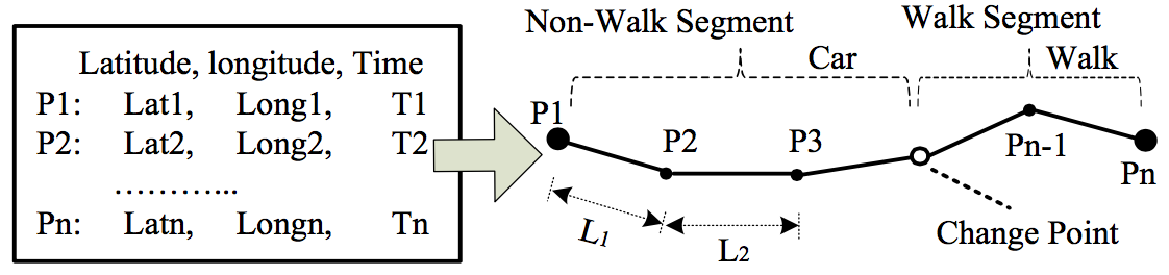
\includegraphics[width=0.5\textwidth]{tm1.pdf}
\caption{GPS logs and transportation mode prediction~(From~\cite{Zheng:2008:UMB:1409635.1409677})}
\end{figure}

\subsubsection{Contributions}

\paragraph{Results\newline}

In order to infer the transportation mode, the authors identify a set of novel features beyond 
simple velocity and acceleration. These features along with a post processing algorithm are 
robust to the traffic condition and contain significant information of users motion. The technique 
was evaluated using GPS logs collected by 65 users over a time period of 10 months. The authors 
evaluated the proposed approach by considering various combinations of the suggested features
and achieved a prediction accuracy of 72.8~\%.   

\paragraph{Approach\newline}

The framework to infer the transportation mode consists of an offline learning stage and a online
processing stage. In the offline learning part, the GPS trajectories are partitioned into segments
depending on the direction change points. The individual segments are than utilised to extract 
several features which are used to train a classification model for the online inference stage.\newline

When the GPS trajectory comes, it is first partitioned into segments from which several features such as 
direction change rate, velocity change rate, stop rate and heading direction are extracted. 
Using these features, the inference model is utilised to predict the transportation mode for
a given segment in a probabilistic manner. As a classification model, decision tree is used based on 
a change point based segmentation method. The change points are grouped into several clusters using
a density-based clustering algorithm. The derived clusters are used to construct an undirected graph
with nodes as individual cluster and edges being the transportation between nodes. A spatial index is
built over the graph to improve the efficiency of accessing information of each node and edge. Finally,
the probability distribution is calculated of different transportation modes on each edge.    

change point based segmentation method, variable traffic conditions, graph based post processing 
algorithm, independent of any additional database of road networks or POI's. Independent of sensor data
such as GSM signal, heart rate, and map information like road networks and bus stops. Therefore
can be deployed in a range of web applications. Non user-specific model. 


\subsection{Discussion} \label{lect1-disc}

The major contribution of the above paper is a methodology to infer the mobility mode given raw GPS
data logs.    


\begin{itemize}

\item An important limit of GPS system is its battery life. During the recording step of this work, the user could not anticipate the recharging because there was no visible indication of the battery power level of the GPS system. This problem explains why gaps exist in the data collection and may influence the accuracy of the model created.

\item The data collection is only related to a single user. At the beginning of the paper, some multi-user applications are described and it would have been interesting to build predictive models for several users, in order to link or to compare them in a multi-user application.

\item The absence of time dimension might be a limit because it is not included in the prediction, while time might have an important impact on the user's movements. Consequently, the Markov model should be extended in order to add this crucial information.

\item If the user changes her habits (home or work place), it is impossible to be sure that the Markov model is really up to date. We could add a threshold and a counter in the algorithm in order to highlight changes and relevant new paths.

\item Finally, it is very important to build a model but it is also important to validate it in order to demonstrate that the model is relevant. However, a validation section misses in this paper. For example, this validation section could be detailed with some queries realized on the system in order to show the level of accuracy or margin or error of the predictive model.

\end{itemize}